\documentclass[tikz,border=12pt]{standalone}
\usepackage{tikz}
\usetikzlibrary{arrows.meta,calc,decorations.pathreplacing}

\definecolor{inkdark}{HTML}{1E2530}
\definecolor{laserred}{HTML}{D93A3A}
\definecolor{beamorange}{HTML}{E08A2E}
\definecolor{beamviolet}{HTML}{7A5AA8}
\definecolor{opticblue}{HTML}{2E5E8E}
\definecolor{mirrorgray}{HTML}{4A5560}
\definecolor{panelbg}{HTML}{EEF1F5}
\definecolor{fringeteal}{HTML}{2A8C8C}
\definecolor{softgray}{HTML}{9AA4B0}

\begin{document}
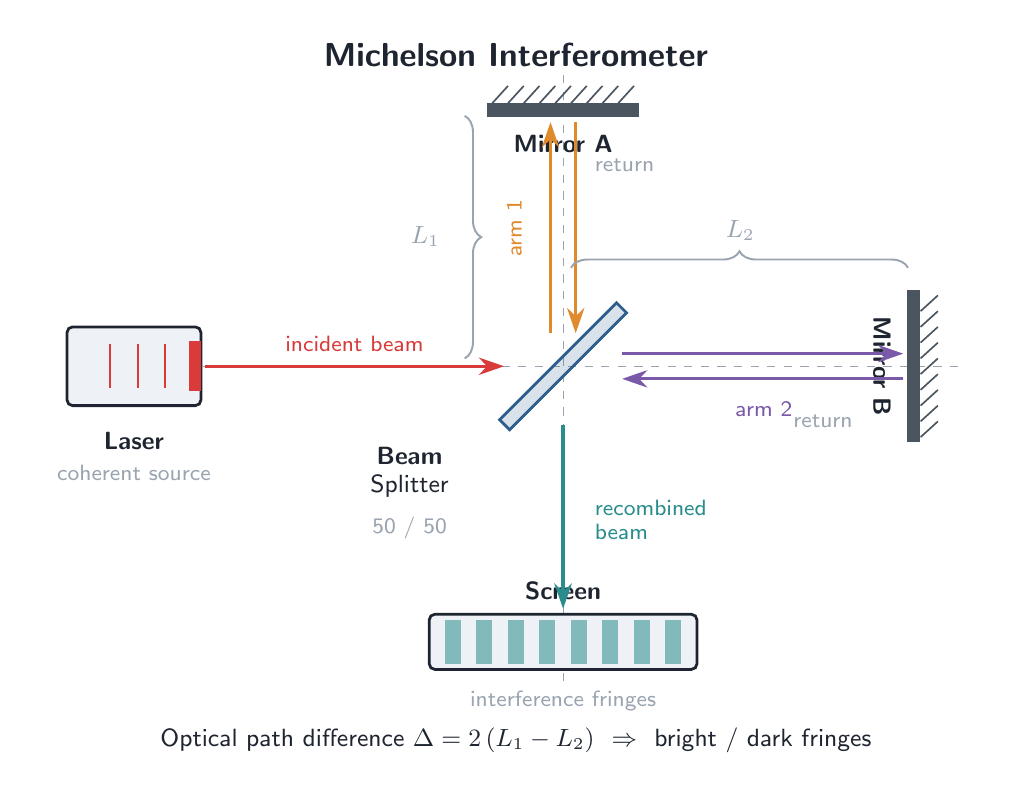
\begin{tikzpicture}[
  every node/.style={font=\sffamily},
  beam/.style={line width=1.1pt,-{Stealth[length=3.2mm,width=2.2mm]}},
  optic/.style={draw=opticblue,line width=1pt},
  lbl/.style={font=\sffamily\small,text=inkdark},
  sublbl/.style={font=\sffamily\footnotesize,text=softgray}
]

% ---- canvas (keeps a 4:3 style framing) ----
\path (-6.8,-5.0) rectangle (5.6,4.3);

% ---- title ----
\node[font=\sffamily\bfseries\large,text=inkdark] at (-0.6,3.95)
  {Michelson Interferometer};

% ---- optical axis guides ----
\draw[softgray,dashed,line width=0.4pt] (-5.0,0) -- (5.1,0);
\draw[softgray,dashed,line width=0.4pt] (0,-4.0) -- (0,3.7);

% ---- Laser source ----
\fill[panelbg,draw=inkdark,line width=1pt,rounded corners=2pt]
  (-6.3,-0.5) rectangle (-4.6,0.5);
\fill[laserred] (-4.75,-0.32) rectangle (-4.6,0.32);
\foreach \i in {1,2,3}{
  \draw[laserred,line width=0.7pt] (-6.1+0.35*\i,-0.28) -- (-6.1+0.35*\i,0.28);
}
\node[lbl] at (-5.45,-0.95) {\bfseries Laser};
\node[sublbl] at (-5.45,-1.35) {coherent source};

% ---- Beam Splitter (50/50 plate at 45 deg) ----
\begin{scope}[rotate=45]
  \fill[opticblue,opacity=0.18] (-1.05,-0.09) rectangle (1.05,0.09);
  \draw[optic] (-1.05,-0.09) rectangle (1.05,0.09);
\end{scope}
\node[lbl,align=center] at (-1.95,-1.35) {\bfseries Beam\\[-1pt] Splitter};
\node[sublbl] at (-1.95,-2.05) {50 / 50};

% ---- Mirror A (top arm) ----
\fill[mirrorgray] (-0.95,3.18) rectangle (0.95,3.32);
\draw[mirrorgray,line width=1pt] (-0.95,3.18) rectangle (0.95,3.32);
\foreach \x in {-0.9,-0.7,...,0.75}{
  \draw[mirrorgray,line width=0.6pt] (\x,3.34) -- (\x+0.2,3.56);
}
\node[lbl] at (0,2.82) {\bfseries Mirror A};

% ---- Mirror B (right arm) ----
\fill[mirrorgray] (4.38,-0.95) rectangle (4.52,0.95);
\draw[mirrorgray,line width=1pt] (4.38,-0.95) rectangle (4.52,0.95);
\foreach \y in {-0.9,-0.7,...,0.75}{
  \draw[mirrorgray,line width=0.6pt] (4.54,\y) -- (4.76,\y+0.2);
}
\node[lbl,rotate=-90] at (4.05,0) {\bfseries Mirror B};

% ---- Screen / detector ----
\fill[panelbg,draw=inkdark,line width=1pt,rounded corners=2pt]
  (-1.7,-3.85) rectangle (1.7,-3.15);
\foreach \x in {-1.5,-1.1,-0.7,-0.3,0.1,0.5,0.9,1.3}{
  \fill[fringeteal,opacity=0.55] (\x,-3.78) rectangle (\x+0.2,-3.22);
}
\node[lbl] at (0,-2.85) {\bfseries Screen};
\node[sublbl] at (0,-4.25) {interference fringes};

% ---- Beams ----
% incoming
\draw[beam,laserred] (-4.55,0) -- (-0.75,0);
\node[sublbl,text=laserred,above] at (-2.65,0.06) {incident beam};

% BS -> Mirror A (up) and back
\draw[beam,beamorange] (-0.16,0.42) -- (-0.16,3.10);
\draw[beam,beamorange] (0.16,3.10) -- (0.16,0.42);
\node[sublbl,text=beamorange,align=center,rotate=90] at (-0.62,1.75) {arm 1};

% BS -> Mirror B (right) and back
\draw[beam,beamviolet] (0.75,0.16) -- (4.32,0.16);
\draw[beam,beamviolet] (4.32,-0.16) -- (0.75,-0.16);
\node[sublbl,text=beamviolet] at (2.55,-0.55) {arm 2};

% recombined beam -> screen
\draw[beam,line width=1.6pt,fringeteal] (0,-0.75) -- (0,-3.08);
\node[sublbl,text=fringeteal,align=left,anchor=west] at (0.28,-1.95)
  {recombined\\[-1pt] beam};

% ---- direction hints on the returning paths ----
\node[sublbl,anchor=west] at (0.28,2.55) {return};
\node[sublbl,anchor=south] at (3.3,-0.9) {return};

% ---- arm length braces ----
\draw[decorate,decoration={brace,amplitude=6pt},softgray,line width=0.7pt]
  (-1.25,3.18) -- (-1.25,0.10);
\node[lbl,text=softgray] at (-1.75,1.65) {$L_1$};

\draw[decorate,decoration={brace,amplitude=6pt},softgray,line width=0.7pt]
  (0.10,1.25) -- (4.38,1.25);
\node[lbl,text=softgray] at (2.25,1.72) {$L_2$};

% ---- caption ----
\node[font=\sffamily\small,text=inkdark] at (-0.6,-4.75)
  {Optical path difference $\Delta = 2\,(L_1 - L_2)$\ \ $\Rightarrow$\ \ bright / dark fringes};

\end{tikzpicture}
\end{document}
